\documentclass[10pt,twocolumn,letterpaper]{article}

\usepackage{cvpr}
\usepackage{times}
\usepackage{epsfig}
\usepackage{graphicx}
\usepackage{amsmath}
\usepackage{amssymb}

% Include other packages here, before hyperref.

% If you comment hyperref and then uncomment it, you should delete
% egpaper.aux before re-running latex.  (Or just hit 'q' on the first latex
% run, let it finish, and you should be clear).
\usepackage[pagebackref=true,breaklinks=true,letterpaper=true,colorlinks,bookmarks=false]{hyperref}

% \cvprfinalcopy % *** Uncomment this line for the final submission

\def\cvprPaperID{****} % *** Enter the CVPR Paper ID here
\def\httilde{\mbox{\tt\raisebox{-.5ex}{\symbol{126}}}}

% Pages are numbered in submission mode, and unnumbered in camera-ready
\ifcvprfinal\pagestyle{empty}\fi
\begin{document}

%%%%%%%%% TITLE
\title{Visual Census Using Cars}

\author{First Author\\
Institution1\\
Institution1 address\\
{\tt\small firstauthor@i1.org}
% For a paper whose authors are all at the same institution,
% omit the following lines up until the closing ``}''.
% Additional authors and addresses can be added with ``\and'',
% just like the second author.
% To save space, use either the email address or home page, not both
\and
Second Author\\
Institution2\\
First line of institution2 address\\
{\tt\small secondauthor@i2.org}
}

\maketitle
%\thispagestyle{empty}

%%%%%%%%% ABSTRACT
\begin{abstract}
Detecting a large number of BMWs in images informs us that those images may be of a wealthy area. Conversely, knowing that our images were obtained from a wealthy neighborhood increases the likelihood of detecting expensive cars. We explore this relationship between demographic factors and fine-grain classes by performing large scale detection of over 2600 car classes and conducting a social analysis of unprecedented scale in computer vision. Using 45 million images from 200 of the biggest cities in the United States,we predict demographic factors such as neighborhood wealth and crime statistics. Finally we show that just as fine-grain classes provide demographic information, societal cues can assist in fine-grain classification and improve accuracy. To facilitate our work, we have collected the largest and most challenging fine-grain dataset reported to date consisting of 3147 classes of cars comprised of images from google street view and other web sources and classified by car experts to account for even the most subtle of visual differences. We hope our work ushers in a new research area fusing fine-grained object detection and societal analysis.
\end{abstract}

\section{Introduction}
%%%%%%%%% BODY TEXT
The ubiquity of street view images has jumpstarted a new line of computer vision research focused on understanding cities through images \cite{mit_plos_1}~\cite{MIT_vision}~\cite{tamara}. For example, \cite{mit_plos_1} showed that crime predictions can be improved by incorporating human perceptions of neighborhoods' images rather than using census data such as income alone~\cite{mit_plos_1} and ~\cite{tamara} and \cite{MIT_vision} learn these perceptions using computer vision techniques. However, in order to extend these methods to other cities,extensive annotations of millions of images from each city would be required since, as ~\cite{tamara} showed, algorithms trained on images of Boston, for example, cannot predict safety or wealth on images from San Francisco.  We explore the question of learning social priors using large scale fine-grain classifications of cars and show that many neighborhood statistics such as income and crime rate can be predicted from car detections. Furthermore, using our detections in conjunction with census data, we can answer questions like what types of cars do rich/poor people drive? 

\begin{figure}[t]
\begin{center}
\fbox{\rule{0pt}{2in} \rule{0.9\linewidth}{0pt}}
   %\includegraphics[width=0.8\linewidth]{egfigure.eps}
\end{center}
   \caption{some pull figure}
\label{fig:pull}
\end{figure}

\label{fig:dataset1}
\begin{figure*}[t]
\begin{center}
   \includegraphics[width=0.435\linewidth]{img/web.png}
   \includegraphics[width=0.475\linewidth]{img/streetview.png}
\end{center}
   \caption{Left: examples of cars from craigslist, cars.com and edmunds.com, Right: examples of cars from streetview images. Cars from streetview images are blurred and occluded.}
\end{figure*}

Finally we show that we can use the answers to these questions to help improve fine-grained classification. Although an increasing number of images that we interact with daily are associated with GPS tags, there are very few computer vision algorithms that take advantage of location based metadata. This metadata can be especially important in fine grain classification. For example, just as detecting a large number of expensive cars in one area can give us a hint that we are in the vicinity of a wealthy neighborhood, knowing that we are in a wealthy neighborhood can also increase our likelihood of detecting expensive cars. Similarly, knowing that we are in a farm area increases our likelihood of detecting farm related cars and seeing many family households with young children increases our likelihood of detecting SUVs. We show that this information can be leveraged to improve fine-grain classification. Although there has been previous work on learning spatio-temporal priors for fine-grain classification~\cite{birdsnap} and exploiting street view geometry and GIS systems to improve object detection~\cite{nyc3D,amir} to our knowledge this is the first time census data and other social cues have been used to assist in fine-grain classification.  


Summarizing our contributions:
  \begin{enumerate}
    \item We perform a large scale analysis of cities using our car detections and present intuitive as well as interesting insights
    \item We show that using social cues extracted from census data can improve fine-grain classification accuracy
    \item We present the largest fine-grain car dataset reported to our knowledge, complete with geotags and class as well as geography metadata  
    \item We include a larger set of 45 million street view images with car detections and fine-grain class predictions
  \end{enumerate}

%------------------------------------------------------------------------

\section{Related Work}
\textbf{Analysis of cities using images.}
  \begin{enumerate}
     \item Plos one journal from MIT asking people to predict whether an area is safe/wealthy etc... after looking at the images
     \item streetscore MIT paper predicting safety wealth scores etc.. just from images~\cite{MIT_vision}
     \item tamara Berg's paper on safety on ECCV
     ~\cite{zhang2014part}
     ~\cite{caltech_birds}

\textbf{Using GPS data to improve object detection.}
     \item Amir's work in GIS assisted object detections. For objects like streetlamps and trashcans, uses GIS to reproject objects to a plane and reduce the search space for object detection .
     \item NYC 3D uses geographic elevation data to create view-point aware detectors and extract ground planes for  them
     \item Birdsnap fine-grain dataset with spatio-temporal prior for birds

  \end{enumerate}

%------------------------------------------------------------------------
\section{Data}
\label{sec:dataset}
In order to find out how much we can learn about cities by analyzing cars detected from street view images we need to:
  \begin{enumerate}
    \item Collect a very dense number of street view images from the cities that we are interested in. If the sampling is not dense enough, our conclusions may not be valid or arise because of sampling error.
    \item Gather a large dataset of cars that contains most of the cars that we would find in the US so that we can train a car detector and classifier. 
    \item Gather census and demographic data for the location of each street view image.
  \end{enumerate}
  We briefly discuss 1. and 2. in this section.
We first collected 45 million images from 8 million lat,longs by sampling roads every 25m. For each lat,long we have images at 0, 60, 120, 180, 240, 300 degree rotations. In order to train a fine-grained car classifier to detect and classify the cars in our gathered images, we created the largest ever reported fine-grained dataset of cars consisting of all the cars listed on edmunds.com (all cars manufactured after 1990). In order to create this dataset, we first created a class list using edmunds.com by obtaining example images of all the cars they have (18017 cars) and grouped the cars into visually indistinguishable classes using a series of amazon mechanical turk tasks as well as manual labor by the authors. This resulted in 3147 visually indistinguishable classes. We then collected additional images of cars from cars.com and craigslist. Using AMT, we labeled 400k of these images and 200k of our streetview images with bounding boxes for cars. 

Finally, we hired car experts to label the cars in 100k of our  street view images, classifying them into one of the 3147 calsses that we created. We also labeled the cars from craigslist and cars.com by parsing the car posting titles. The final car dataset consists of 500k images consisting of 200k street view images and 300k images from craigslist.com, cars.com and edmunds.com. We split our data into training, validation and test sets where our training set contains 199,666 streetview images and 313,099 web images, and the validation and test sets contain 39,933 and 159,732 streetview images respectively. Although we are interested in classifying street view images, having web images in our training set increases the amount of data we have without paying expensive car experts to annotate street view images. Fig.~\ref{fig:dataset2} shows some examples of cars from our dataset. We can see that cars from street view images are generally occluded and blurry where as cars from other web sources have higher resolution and are unoccluded.


\section{Detecting and classifying cars}
After collecting images and creating a dataset, we have to train a car detection and classification algorithm. Although we would have ideally used the recent RCNN from~\cite{rcnn} due to its state of the art results, the computational and memory requirements of RCNN make it impractical for use in such a large scale detection setting such as ours. Since our training set consists of XXX images and we want to detect cars in \(\sim\)45 million images, scalability\textemdash not only accuracy\textemdash becomes an imortant consideration. Specifically, training an RCNN detector on our data would require roughly XXGB of memory and XXX seconds. And detecting cars during test time would take \(\sim\)20s per image which is impractical for detecting multiple cars in \(\sim\)45 million images. Thus our pipeline, instead, consists of using DPM~\cite{dpm} to detect cars and a CNN ~\cite{alexnet} to classify them. We present details in the sections below.

\subsection{Car Detection}
As mentioned above, we not only have to worry about accuracy but also scalability. Thus, we experimented with different DPMs to evaluate accuracy/speed trade off. A single component DPM with 8 parts gives us the best tradeoff between accuracy and speed and our supplemental material discusses many other configurations that we have tried. For example, a DPM with 1 component and 8 parts results in an average precision (AP) of 64.2\% and takes 5 seconds per image at test time where as a DPM with 3 components and 8 parts results in 68\% AP and takes \(\sim\)15 sec per image. The highest AP that we measured was a value of 68.7\% with a 5 component 8 parts model that takes \(\sim\)22 sec per image. 

\begin{figure} [t]
\begin{center}
\includegraphics[width=0.8\linewidth]{img/car_hierarchy.jpg}
\end{center}
\caption {Car class hierarchy. Classes are usually more visually similar when we travel down the tree.}
\label{fig:hierarchy}
\end{figure}

\begin{table}
\begin{center}
\begin{tabular}{|l|c|}
\hline
\textbf{Attribute} & \textbf{Acc\%} \\
\hline\hline
Make & 55 \\
Model & 60 \\
Submodel & 70 \\
Year (5 bins) & 40 \\
Price (5 bins)& 50 \\
Domestic/Foreign & 80\\
Country & 80\\
\hline
\end{tabular}
\end{center}
\caption{Accuracy by car attribute}
\label{table:tree-acc}
\end{table}

\begin{figure*} [t]
\begin{center}
\includegraphics[width=0.55\linewidth]{img/good_det.png}
\raisebox{-0.02\height}
 {
\includegraphics[width=0.34\linewidth]{img/cars.jpg}
 }
\end{center}
\caption {An example of our car detections and classifications. The red boxes are DPM bounding boxes that are not classified and green boxes are classifications. The two cars in the image are correctly classified to the classes shown on the right.}
\label{fig:dets}
\end{figure*}

\subsection{Car Classification}
After doing car/no car detection, we use a standard CNN from ~\cite{alexnet} with ~\cite{caffe} to classify the cars into one of 2657 fine-grained classes. Although we want to classify cars from street view images, as mentioned in sec.~\ref{sec:dataset} XX\% of our training images consist of cars from other sources such as craigslist due to the fact that annotating street view images is much more expensive. Thus we add deformations such as blurring in an attempt to make the non-street view images look like street view images. We give details of training the CNN in our supplementary material. At test time we take the top 10\% scoring DPM bounding boxes and classify them. This gives a 10x increase in speed but only a 0.X\% drop in AP as compared to using all the boxes detected by DPM. We achieve an accuracy of 33.X\% on the true positive DPM bounding boxes and 31.27\% on the ground truth bounding boxes. Fig.~\ref{fig:good_dets} shows an example of our streetview detections. Surprisingly, the cars are detected and classified correctly even though blurriness and occlusions in street view images makes this a difficult task.

\subsection{Analyzing Hierarchical Classification Accuracy}
Although we are classifying to one of 2657 fine-grained classes, some types of mistakes are more costly for our task of social analysis than others. For example, we might not care about misclassifying 2001 Honda Accord lx to 2001 Honda Accord dx but a mistake classifying a 2012 BMW 3-series to a 1996 Honda Accord would create large errors in our analysis if we, for example, want to estimate the average price or age of a car in a zip code and measure how it is related to median household income. Similarly, misclassifying an SUV to a sedan would confound an analysis estimating the cities with the most number of large cars. Inorder to gain insight into our classification errors we perform a hierarchical accuracy analysis. 

Fig.~\ref{fig:hierarchy} shows one of a few possible car hierarchies. The leaves are the fine-grained classes and the parents are composite classes consisting of the children. Cars become more and more visually indistinguishable while travelling down the tree, with the most similar classes,in most cases, being the leaves sharing a parent. Can you tell the difference between class 1 and class 2? Given the difficulty of our dataset, we were very surprised by the 31.27\% accuracy of our classifier at the leaf level. Table~\ref{table:att-acc} lists accuracies by various car attributes such as those in~\ref{fig:hierarchy} and others like car price, year etc\ldots We can see that the accuracy is much higher after aggregating by different attributes. 


\section{Societal analysis}
\label{sec:social}
After collecting data, training fine-grained car detectors and classifying cars in all of our images, we now have all the components to perform social analysis. We show some general results from the entire united states as well as case studies from cities we could obtain ground truth data for. We divide our analysis into different sections below.

\subsection{What cars on the street tell us about people}

\subsubsection{Cars on the street versus cars people drive}
The first question we asked is how do cars on the street relate to the cars that people drive? Specifically,
can we learn about the registered cars in a zip code from our street view detections?
In order to answer this question we downloaded the vehicle census from Massachusetts, which is the only state to release extensive vehicle registration data. Surprisingly, we found an extremely high Pearson correlation coefficient of 0.9 (p value=XXX) between the number of cars we detected per zip code and the number of cars that are registered per zip code in the three cities we analyzed in Massachusetts: Boston, Worcester and Springfield. The high correlation was only obtained after aggregating cars at the zip code level which tells us that most people in these cities must drive within their zip code. 
After establishing a high correlation between the number of cars we detect and the number of registered cars, we also measured the correlation between the make of the detected and registered cars per zip code. As we can see in fig.~\ref{fig:ma_corrs} there is a high correlation for most of the makes. This shows us that the cars we detect from street view images can actually tell us a lot about the types of cars that people in a particular zip code drive.

\begin{figure} [t]
\begin{center}
\includegraphics[width=1\linewidth]{img/boston_make_corr.png}
\end{center}
\caption {Pearson correlation coefficient and p values between the number of detected and registered cars in Boston for each make.}
\label{fig:ma_corrs}
\end{figure}


\begin{figure}[t]
\begin{center}
   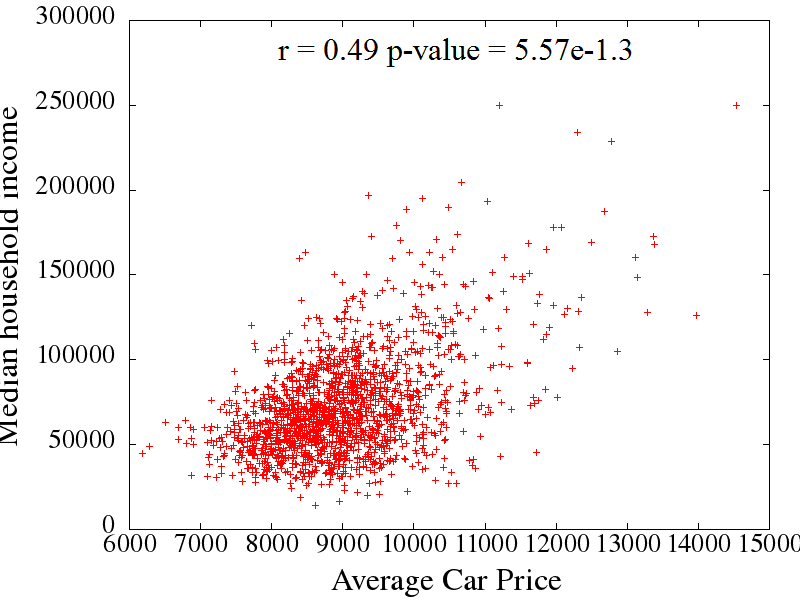
\includegraphics[width=0.8\linewidth]{img/averagePriceIncome.png}
\end{center}
   \caption {Median household income per zip code vs average price of detected cars per zip code.}
\label{fig:price-income-corr}
\end{figure}

\subsubsection{What do rich/poor people drive?}
We gathered zip code level as well as census tract level 2007-2012 American Community Survey data for the 200 cities in our dataset and analyzed how the census data relates to statistics from our detected cars. 

Table \ref{table:car-census-corrs} shows correlation values between various attributes of the detected cars and median household income as well as education level per zip code. Fig.~\ref{fig:price-income-corr} shows a plot of median household income vs. average car price in a zip code. As expected, there is a high correlation between median household income and the average car price per zip code (r=0.49, p \(\sim\) 0). This makes sense since rich people mostly live around places with expensive cars and tend to drive expensive cars. Our results also indicate that rich people prefer to drive foreign, especially German, cars (r=0.59). This observation is also consistent with our expectations since expensive cars such as BMWs are German. What is perhaps surprising is that there is a very high negative correlation (r=-0.55, p \(\sim\) 0) between the percentage of American cars in a zip code and median household income. So poor people live in places with many American cars.

Poor people also live near very old cars where as rich people live near newer ones. As table \ref{table:car-census-corrs} shows, the correlation between median household income and the number of cars in 1990-1994 is very negative and increases to a high positive 0.59 for cars in the 2005-2009 range. Finally, a perhaps not surprising result is that poor people live near cars with low miles per gallon (MPG). This corroborates~\cite{cal-traffic-study} study showing that poor people are more exposed to car pollution than rich people.
 
\begin{figure}[t]
\begin{center}
    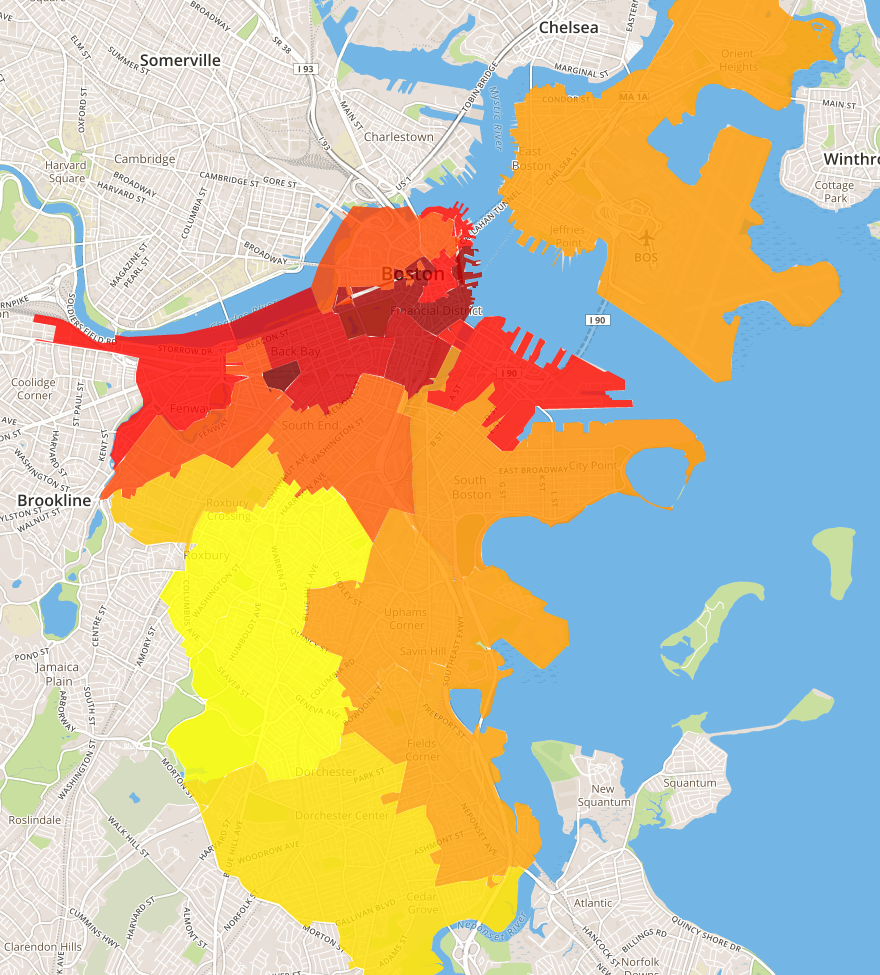
\includegraphics[width=0.45\linewidth]{img/price.png}
    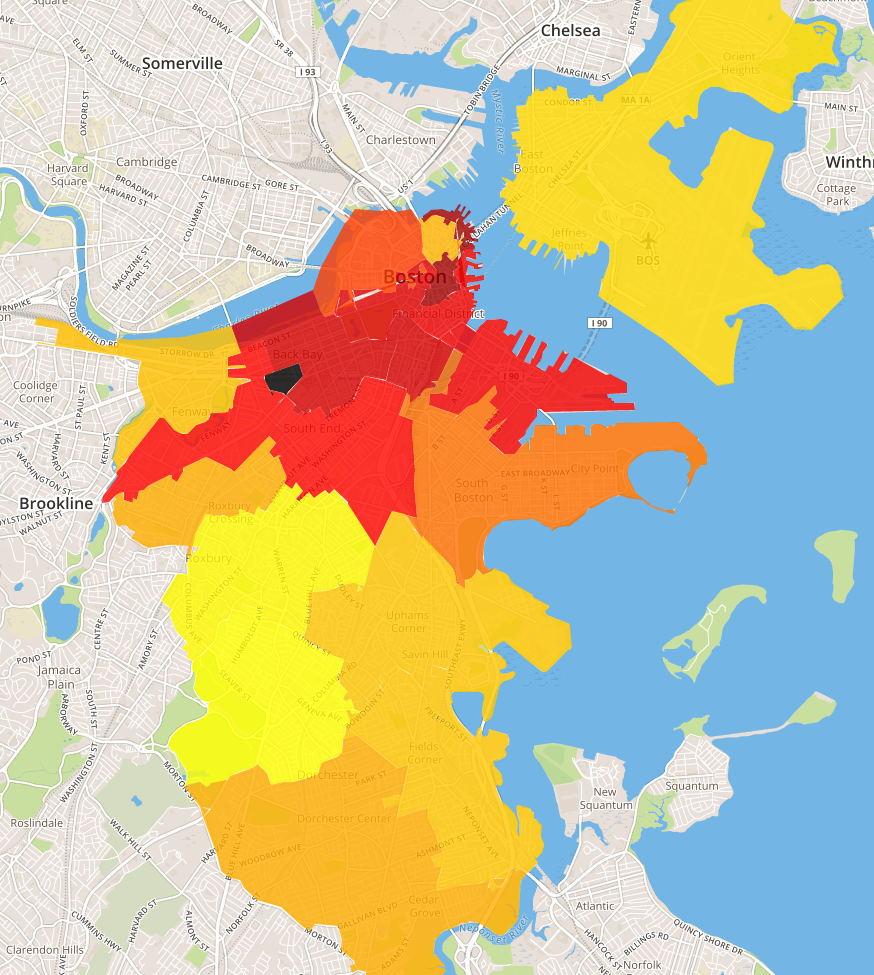
\includegraphics[width=0.45\linewidth]{img/income.png}
  \raisebox{-.5\height}{
    \includegraphics[width=0.45\linewidth]{img/houston_price.png}
    \includegraphics[width=0.45\linewidth]{img/houston_income.png}
  }
\end{center}
   \caption {Top left: Heat map of average car price in Boston, right: heat map of median household income in Boston. Bottom left: Heat map of average car price in Houston, right: heat map of median household income in Houston}
\label{fig:bos-sf-vis}
\end{figure}

\subsubsection{How does education relate to cars on the street?}
One would probably guess that there is a high negative correlation between the number of people with only a high school education and the average price of a car in a zip code. Indeed, we found that this is the case (r=0.3 p \(\sim\) 0). As expected, we also found a high correlation between the number of college educated people in a zip code and the average car price. What is perhaps surprising is that although there is a large increase in correlation coefficient as we go from high school to college educated, the jump from college to graduate school is very low (r=0.31 for college educated and 0.39 for graduate school). This tells us that there is a very low difference in the price of cars driven by people who only hold bachelors as opposed to graduate degrees.

\begin{figure*}[t]
\begin{center}
  \raisebox{-.02\height}
 {
   \includegraphics[width=0.3\linewidth]{img/sf_density.png}
 }
   \includegraphics[width=0.3\linewidth]{img/sf_mpg.png}
   \includegraphics[width=0.3\linewidth]{img/sf_air_cropped.png}
\end{center}
   \caption {A. Density of cars in San francisco inversely weighted by their expected MPG, B. The weighted average of car MPG in San Francisco. The weights are the expected number of cars, C. Ground Truth for Air quality (measured in annual particulate matter) in San Francisco.}
\label{fig:pollution}
\end{figure*}

\begin{table}
\begin{center}
\begin{tabular}{|l|c|r|}
\hline
\textbf{Census Variable} & \textbf{Car Attribute} & \textbf{r}  \\
\hline\hline
Household income & No. 1990-1994 cars & -0.42 \\
Household income & No. 1995-1999 cars & -0.40 \\
Household income & No. 2000-2004 cars & 0.21 \\
Household income & No. 2005-2009 cars & 0.46 \\
Household income & \% foreign cars & 0.59 \\
Household income & \% German cars & 0.57 \\
Household income & \% Us cars & -0.59 \\
Household income & Avg. price & 0.49 \\
Education: highschool & Avg. price & -0.21 \\
Education: college & Avg. price & 0.32 \\
Education: graduate scl. & Avg. price & 0.39 \\
\hline
\end{tabular}
\end{center}
\caption{Pearson correlation coefficient between various census variables and detected car attributes. All p values are \(\sim\) 0.}
\label{table:car-census-corrs}
\end{table}

\subsection{What cars on the street tell us about neighborhoods}
\subsubsection{Which neighborhoods are wealthy/poor?}
We ask the question: what can our street view car detections tell us about the wealth of a neighborhood? Specifically, can we predict which neighborhoods are wealthy or un-wealthy using our detections? Intuitively, if we see many expensive cars on the street, we suspect that we are in a rich neighborhood and vice versa. However, the correlation between car prices and neighborhood wealth is not going to be perfect because we are not necessarily detecting the cars that are registered by residents. Figure \ref{fig:bos-sf-vis} A shows a heat map of the average price of detected cars within a zip code and median household income in a zip code for Boston and figure \ref{fig:bos-sf-vis} B shows the same visualization for Houston. We can see that in both cities, the average car price in a zip code is a very good predictor of wealthy/un-wealthy neighborhoods.


\subsubsection{Which neighborhoods have high car pollution?}
Can our street view detections tell us anything about which neighborhoods are affected by highly polluting cars? To answer this question, we plotted a heat map of the expected number of cars per sample inversely weighted by the expected MPG of that sample as well as the weighted average of car MPG where the weights are the expected number of cars. The first measure should give us a rough idea of the location of highly polluting neighborhoods: for the same density of cars, areas with high MPG result in lower numbers than those with low MPG. For different densities of cars, the relative magnitude of the measure depends on both the density of cars and how efficient they are. The second measure, on the other hand, visualizes areas with a high concentration of low MPG cars.

Fig.~\ref{fig:pollution}A shows the weighted density of cars in San Francisco and B shows the weighted MPG. Although we could not find ground truth data of car pollution, Fig.~\ref{fig:pollution}C is a map of San Francisco air quality measuring annual average particulate matter concentration (MPG) from all sources. To our surprise, their map seems to agree with Fig.~\ref{fig:pollution}B in most cases.


\subsection{What cars on the street tell us about cities}
\subsubsection{Which cities are more segregated?}
In this section we ask the question: which cities show high clustering of similarly priced cars? Specifically, which cities have expensive cars clustered together with other expensive cars and cheap cars clustered with other cheap cars? Given the high correlation between median household income and average car price, the answer to this question should give us a good indication of the cities that are most and least segregated. Following the analysis of ~\cite{mit_plos_1} we use the Moran I statistic to measure spatial autocorrelation where a value of 1 indicates perfect clustering of similar values, -1 indicates perfect dispersion and 0 indicates a random spatial arrangement (neither clustering nor dispersion). Fig.~\ref{fig:moran-i} plots the highest and lowest scoring cities as well as well as few others in between. We can see that Houston shows the highest clustering where as Las Vegas shows the lowest.

\begin{figure}[t]
\begin{center}
    \includegraphics[width=0.8\linewidth]{img/moran_i_red.pdf}
\end{center}
   \caption {Moran I scores for 5 cities. Houston has the highest score where as Las Vegas has the lowest}
\label{fig:moran-i}
\end{figure}

\subsubsection{Which cities are more patriotic?}
Which cities have the most number of domestic cars? As Fig.~\ref{fig:city_price}A shows the coastal cities have a high concentration of foreign made cars where as the midwest has a low concentration. This result is to be expected since the coasts also have a higher number of immigrants as well as a higher concentration of wealthy people. And as we showed in our previous analyses, wealthy people tend to drive foreign cars. The city with the highest percentage of foreign cars was found to be San Francisco where as Casper Wyoming had the least percentage.

\subsubsection{Which cities are wealthier?}
In our final analysis, we ask which city has the most expensive cars on average? Fig.~\ref{fig:city_price}B maps the average car price for each city. We can see that many of the east coast cities have expensive cars as well as some cities in the south like Atlanta. We found the city with the most expensive cars to be New York and the one with the least expensive cars to be El Paso. The fact that our results predict New York may not be surprising given that some of the wealthiest people in the United States live there and those who are less wealthy tend to take public transportation.

\begin{figure*}[t]
\begin{center}
    \includegraphics[width=0.49\linewidth]{img/city_foreign.png}
    \includegraphics[width=0.49\linewidth]{img/city_price.png}
\end{center}
   \caption {A. Map of the percentage of foreign cars in each city. San Francisco has the highest percentage and Casper the lowest. B. Map of the United States showing the expected car price in each city. New York has the highest expected car price where as El Paso has the lowest.}
\label{fig:city_price}
\end{figure*}

\begin{table}
\begin{center}
\begin{tabular}{|l|c|}
\hline
\textbf{Attribute} & \textbf{Acc\%} \\
\hline\hline
Make & X \\
Model & X \\
Submodel & X \\
Year (5 bins) & X \\
Price (5 bins)& X \\
Domestic/Foreign & X\\
Country & X\\
\hline
\end{tabular}
\end{center}
\caption{Gain in fine-grained accuracy with ground truth attributes.}
\label{table:ground}
\end{table}

\begin{table}
\begin{center}
\begin{tabular}{|l|c|c|r|}
\hline
\textbf{Attribute} & \textbf{Census Variable}& \textbf{acc-fg} &\textbf{acc-m}\\
\hline\hline
Price & Median hh income & X & X\\
Year  & Median hh income & X & X\\
Make & No. ppl in Management & X &X \\
Submodel & No. ppl 6-17 years & X & X \\
Domestic & Median hh income & X & X\\
Country & Median hh income & X & X\\
\hline
\end{tabular}
\end{center}
\caption{Census variables resulting in the highest accuracy gain for each car attribute. Acc-fg is the gine-grained accuracy and acc-m is the make level accuracy. Car price/year with median household income give the highest gain in accuracy.}
\label{table:prior-acc}
\end{table}

\section{Using social priors to improve classification}
In section~\ref{sec:social} we showed that street view car detections give a lot of information about people, neighborhoods and cities. In this section we ask the reverse question: does our knowledge of neighborhood demographics teach us something about the cars in that neighborhood? Intuitively, if we know that a particular image was taken in a wealthy neighborhood, for example, we would expect the cars in that neighborhood to be expensive. Can we use this information to improve our car classifications?

To answer this question, we first tried to use zip code level census variables as priors, calculating \(P(C|I,Sk)\) where \(C\) is the fine-grained class, \(I\) is an image and \(Sk\) \(\in\) \(\{\)\(S1\)\ldots \(Sn\)\(\}\)is a particular zip code level census variable such as median household income. After applying Bayes' rule, assuming that the image and census data are conditionally independent given the class label, and applying Bayes' rule again we get:

\begin{equation}
P(C|I,Sk)\propto \frac{P(C|I)}{P(C)}P(C|Sk)
\label{eq:prior-eq}
\end{equation}

Where \(P(C|I)\) is the output of our CNN classifier. A naive way of using census variables such as the one above reduces accuracy by 5.x\% to ~26.x\%. This is not surprising given that we have over ~2500 fine-grained classes, and many of them have similar attributes such as price. We expect census variables to be good indicators of cheap vs. expensive or old vs. new cars but not to give us much information about the presence/absence of cars with similar attributes at the fine-grained level such as 2001 Honda Accord lx vs. 2001 Honda Accord dx. With this insight, instead of using census variables directly as fine-grained class priors, we use them as priors for the car attributes. Table~\ref{table:ground} lists fine-grained accuracy gains after plugging in ground truth attributes. These values give an upper bound for the gain in accuracy that can be achieved after perfectly predicting each attribute. With this in mind, to incorporate the census variables into our classificaion pipeline we can reformulate \(P(C|Sk)\) in equation~\ref{eq:prior-eq} as \(P(C|Aj)\)\(P(Aj|Sk)\) where \(Aj\) \(\in\) \(\{\)\(A1\)\ldots\(An\)\(\}\) represents a car attribute such as price. After this modification, equation~\ref{eq:prior-eq} can be written as  

\begin{equation}
  P(C|I,Sk) \propto \frac{P(C|I)}{P(C)}P(C|Aj)P(Aj|Sk)
\end{equation}
We calculate \(P(C|I,Sk)\) for all car attributes and 30 different census variables, quantizing some car attributes and census variables such as car price and median household income into bins ranging from 2-20. Table~\ref{table:prior-acc} shows the highest accuracy numbers for various combinations of census variables and car attributes. It can be seen that using median household income and either car price or year give the highest accuracy gain. This result is to be expected since, as seen in section~\ref{sec:social}, there is a high correlation between median household income and car price and year. Although the accuracy gain at the fine-grained level is very slight (which is to be expected due to the large number of similar classes in our dataset), we get more significant gains in accuracy at higher levels of the hierarchy such as car make. 

\section{Conclusion}
{\small
\bibliographystyle{ieee}
\bibliography{egbib}
}

\end{document}

{\small
\bibliographystyle{ieee}
\bibliography{egbib}
}
\end{document}


